\section{Description of model equations}

\subsection{Mathematical formulation of a crypt-based model of adenoma initiation}

The paper creates a mathematical model of advanced adenoma formation based on the multi-step oncogenic properties of colorectal cancer. The model is parametrized with experimentally obtained data so the epidemiological predictions can better fit the incidence data that document advanced adenoma occurrence as a function of age. This allows for accurate fine-tuning of the model predictions. 

\begin{figure}[h]
    \centering
    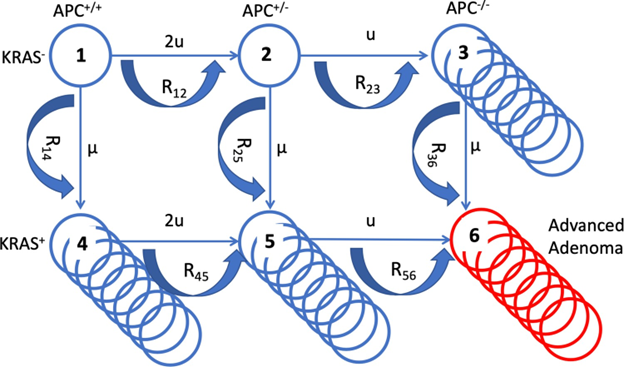
\includegraphics[width=0.65\linewidth]{figures/CancerModel.png}
    \caption{Schematic of the mathematical model. The six cell types are denoted by circles, the mutation rates ($u, \mu$) that give rise to different types are marked by the straight arrows. Type 6 late adenoma is marked in red. Crypt conversion rates ($R_{ij}$) are indicated by circular arrows. Crypt fission ($\gamma_i$) are indicated by multiple circles.}
    \label{fig:A schematic illustrating the mathematical model}
\end{figure}

The associated selection mutation diagram is shown in Figure 1. There are six distinct crypt populations indicated as types 1 through 6.  
The mutation rate between types are specified as follows:

Inactivation of the first copy of the APC gene \( APC^{+/-} \): 
\( u_{1 \to 2} = u_{4 \to 5} = 2u \).

Inactivation of the remaining copy of the APC gene \( APC^{-/-} \): 
\( u_{2 \to 3} = u_{5 \to 6} = u \).

Finally, activation of the KRAS gene \( KRAS^{+} \): 
\( u_{1 \to 4} = u_{3 \to 6} = \mu \).

\( R_{ij} \) is the conversion rate from crypt type \( i \) to type \( j \).

In Figure 1, the populations in the top row, types 1-3, are characterized by an unmutated KRAS oncogene while the populations of the bottom row, types 4-6, have the KRAS mutation activated. Moving from left to right on this diagram, the number of inactivated copies of the APC gene increases from 0 to 2, such that populations of types 1 and 4 are APC$^{+/+}$, populations of types 2 and 5 are both APC$^{+/-}$, and populations of types 3 and 6 are APC$^{-/-}$.


%The mathematical model aims to capture how . 
Corresponding with the possible two mutations in APC and one mutation in KRAS there are a total of 6 different types of crypts.  
The population of each crypt is denoted as $n_i$ with $1 \leq i \leq 6$. 
%*** There is no differential equation for type 6 because?
The rate of population change of each crypt is denoted as $\dot{n}_i$ with $1 \leq i \leq 6$.
$\delta$ is the death rate for crypts and the same for all because these are similar cells. 
$\gamma_i$ is the corresponding growth rate for crypt fission and varies significantly between crypts.
It is reasonable to assume that $\gamma_2 = 0$ , because APC$^{+/-}$ crypts do not divide, and that $\gamma_4 = \gamma_5$ because APC$^{+/+}$ and APC$^{-/-}$ crypts with and without a KRAS mutation divide at the same rate.

%Using the variables previously mentioned, the authors created the following linear differential equations can be created and used to calculate the rate of population change for each type of colonic crypt.

%Linear system
%\begin{equation}
%\begin{cases}
%\begin{aligned}
%    \dot{n}_1 &= -(R_{12} + R_{14})n_1, \\
%    \dot{n}_2 &= R_{12}n_1 - (R_{23} + R_{25})n_2 + \gamma_2n_2,\\
%    \dot{n}_3 &= R_{23}n_2 - R_{36}n_3 + \gamma_3 n_3, \\
%    \dot{n}_4 &= R_{14}n_1 - R_{45}n_4 + \gamma_4 n_4, \\
%    \dot{n}_5 &= R_{25}n_2 - R_{45}n_4 - R_{56}n_5 + \gamma_5n_5\\
%\end{aligned}
%\end{cases}
%\end{equation}
%\[n_1(0) = N_{crypt},\quad n_i(0) = 0, \quad1 \leq i \leq 5.\]


%The paper states it is further possible to ignore the outgoing rates, which simplifies this linear system to the following:
%\begin{equation}
%\begin{cases}
%\begin{aligned}
%    \dot{n}_1 &= 0,\\
%    \dot{n}_2 &= R_{12}n_1 + \gamma_2n_2,\\
%    \dot{n}_3 &= R_{23}n_2 + \gamma_3 n_3,\\
%    \dot{n}_4 &= R_{14}n_1 + \gamma_4 n_4,\\
%    \dot{n}_5 &= R_{25}n_2 + R_{45}n_4 +\gamma_5n_5
%\end{aligned}
%\end{cases}
%\end{equation}
%\[n_1(0) = N_{crypt},\quad n_i(0) = 0, \quad1 \leq i \leq 5.\]

The paper builds on previous models from \autocite{OtherMathModel} by accounting for direct competition between crypts. By assuming that the crypts that undergo crypt fission, types 3, 4, and 5, are in direct competition with each other the equations are changed to models of logistic growth with carrying capacities instead of straight exponential growth. 
Thus the carrying capacities $K_A$ and $K_R$ are added to the differential equations. Where $K_A$ is the the carrying capacity for KRAS$^-$ crypts types 1, 2 and 3. and $K_R$ is the carrying capacity for KRAS$^+$ crypts types 4, 5, and 6. This turns linear differential equations into nonlinear differential equations.
In reference to 
\autocite{OtherMathModel} where no crypt competition was included, such that $K_R = K_A = \infty$ in that model.
Due to nonlinearity an analytical solution is not available. However, a solution procedure similar for a linear system for the nonlinear equations is still possible and can be performed numerically to solve the nonlinear differential equations.

\begin{equation}
\begin{cases}
\begin{aligned}
    \dot{n}_1 &= -(R_{12} + R_{14})n_1, \\
    \dot{n}_2 &= R_{12}n_1 - (R_{23} + R_{25})n_2, \\
    \dot{n}_3 &= R_{23}n_2 - R_{36}n_3 + \gamma_3 n_3 \left( 1- \frac{n_3+n_4+n_5}{K_A} \right) - \delta n_3, \\
    \dot{n}_4 &= R_{14}n_1 - R_{45}n_4 + \gamma_4 n_4 \left( 1- \frac{n_3+n_4+n_5}{K_R} \right) - \delta n_4, \\
    \dot{n}_5 &= R_{25}n_2 - R_{45}n_4 - R_{56}n_5 +  \gamma_5 n_5 \left( 1- \frac{n_3+n_4+n_5}{K_R} \right) - \delta n_5\\
\end{aligned}
\end{cases}
\end{equation}
\[n_1(0) = N_{crypt},\quad n_i(0) = 0, \quad1 \leq i \leq 5.\]

%not sure if this is important for rest of paper.
The probability that by time $t$ at least one crypt of type 6 has been created denoted as $P(t)$, using the mean-field approximation from \autocite{AspirinForTheChemopreventionOfColorectalAdenomas}, is given by the solution of the following equation. This equation can be used to calculate incidence which is discussed later in this paper.
\[ \dot{P}(t) = \left(R_{56}n_5 + R_{36}n_3 \right) \left(1 - P(t) \right), \quad P(0) = 0 \]


%The paper then proceeds to evaluate which pathway towards adenoma formation is most likely. ***
%not sure if important for rest of paper.

\subsection{Model parameters}

The remaining model parameters are defined in this section.
%The mutation rate between types are specified as follows.
%Inactivation of the first copy of the APC gene: \( u_{1 \to 2} = u_{4 \to 5} = 2u \). 
%Inactivation of the remaining copy of the APC gene: \( u_{2 \to 3} = u_{5 \to 6} = u \). 
%Activation of the KRAS gene: \( u_{1 \to 4} = u_{3 \to 6} = \mu \).
The number of stem cells per crypt is denoted as $K$.
The division rate of wildtype stem cells per year denoted ($r_i$). Corresponding to the crypt type number the relative fitness of mutated cells is given as follows.
The relative fitness of \( \text{APC}^{+/-} \) cells is \( F_2 = F_{\text{APC}^{+/-}} \), 
and the relative fitness of \( \text{APC}^{-/-} \) cells is \( F_3 = F_{\text{APC}^{-/-}} \). 
Similarly, the relative fitness of \( \text{KRAS}^{+} \) cells is \( F_4 = F_{\text{KRAS}^+} \). 
The division rate of \( \text{APC}^{-/-} \) \(\text{KRAS}^{-} \) crypts per year is \( \gamma_3 \), and the division rate of \( \text{APC}^{+/+} \)\( \text{KRAS}^{+} \) crypts per year is \( \gamma_4 \). 


The relative fitness of the mutated cells relative to wildtype are given using the cell replacement data from  Komarova et al, using $Pr(j)$ as the probability of replacement of the wild type by type $j$ \autocite{DynamicsOfGeneticInstabilityInSporadicAndFamilialcolorectalCancer}.
%\begin{equation}
%F_j \equiv \frac{r_jd_i}{d_jr_i}=\frac{Pr(j)}{1-Pr(j)} %\quad j \in2,3,4
%\end{equation}

The death rates are assumed to be the same among crypt types, so that $r_i = F_i r_1, \text{ for} \quad 1 \leq i \leq 6.$
Wild-type crypts and those with a single copy of the APC gene do not proliferate so that: 
$\gamma_1 = \gamma_2 = 0.$
Crypts with a KRAS mutation and APC$^{+/+}$ and APC$^{+/-}$ phenotypes proliferate at the same rate so that:
$ \gamma_4 = \gamma_5. $
The conversion rates $R_{ij}$ are given by the equation
$R_{ij} = r_i Ku_{i \to j} \rho_{ij},$
where \( r_i \) is the division rate of type \(i\), \( u_{i \to j} \) is the mutation rate from type \(i\) to type \(j\), and \( \rho_{ij} \) is the probability that one cell of type \(j\) becomes fixated in a compartment of size \(K\) with the host type. 
%To calculate $\rho_{ij}$, let us denote by \(d_i\) the death rate of type \(i\), and $\frac{r_id_j}{r_jd_i}$ as the inverse of the relative fitness of the crypt to get:

The values of each parameter utilized are in the Appendix - Table 4


%\begin{equation}
%\rho_{ij} = \frac{1-\frac{r_id_j}{r_jd_i}}{1-%\left(\frac{r_id_j}{r_jd_i} \right)^K}
%\end{equation}

%Not necessary:
%\noindent \textbf{Fitting the linear model to advanced adenoma incidence data:}

%In order to fit the linear model to the data, the parameters \( N \), \( K \), \( u \), and \( \mu \) were fixed while varying the remaining parameters in stages. First, the fitness parameters (\( F_1 \), \( F_2 \), \( F_3 \)) were fixed to their values as described in (Appendix 1 - Table2), then the parameters (\( r_i \), \( \gamma_3 \), \( \gamma_4 \)) were varied to find the global minimum of error between the model and the data. Then, other select values for the relative fitness parameters (\( F_1 \), \( F_2 \), \( F_3 \)) were taken to show the results remained quantitatively similar. Then, they described the results of fitting and the patterns that were observed.

%To find the global minimum of the error, they varied the parameter \( r_1 \) between once a day and once every twenty days. For each value of \( r_i \), the error was minimized in the 2-dimensional parameter space (\( \gamma_3 \), \( \gamma_4 \)) and a unique minimum was found for every $r_i$. The best fits corresponding to a subset of these division rates are plotted in Appendix 1 - figure 2(a), with the best fitting values shown in Appendix 1 - figure 2(a) panel b for each \( r_1 \).

%From this, we can see that as \( r_1 \) increases, crypt fission rates decrease, and the incidence curves become less steep, until the best fitting crypt fission rate reaches zero. This is when the best fitting incidence curve is achieved because further increase in \( r_1 \) results in an increase that happens too early. 

%In summary, the study found that to minimize the error and best match the observed adenoma incidence, stem cells in the model should divide relatively quickly, about every 1.5 days or faster, and crypt fission should essentially stop. Slower division rates lead to steep, unrealistic predictions of adenoma growth.





%Sentences of Variables
%The number of crypts is denoted as \( N_{\text{crypt}} \), and the number of stem cells per crypt is represented by the symbol \( K \). The rate of inactivation of APC per cell division is given by \( u \), while the rate of activation of KRAS per cell division is denoted by \( \mu \). The division rate of wild-type stem cells per year is \( r_i \). The relative fitness of \( \text{APC}^{+/-} \) cells is \( F_2 = F_{\text{APC}^{+/-}} \), and the relative fitness of \( \text{APC}^{-/-} \) cells is \( F_3 = F_{\text{APC}^{-/-}} \). Similarly, the relative fitness of \( \text{KRAS}^{+} \) cells is \( F_4 = F_{\text{KRAS}} \). The division rate of \( \text{APC}^{-/-} \) crypts per year is \( \gamma_3 \), and the division rate of \( \text{KRAS}^{+} \) crypts per year is \( \gamma_4 \).

